\documentclass{beamer}

\usepackage[francais]{babel}
\usepackage[utf8]{inputenc}
\usepackage[T1]{fontenc}

\usetheme{Warsaw}
\title{Intelligence Artificielle : promesses et réalités}
\author{Ouail Abed - Hackenolz Guillaume - Soufyani Amine}
\date{20 mars 2018}


\begin{document}

	\begin{frame}
	\titlepage
	\end{frame}
	
	\begin{frame} % 2eme transparent TDM générale
	\frametitle{Table des matieres}
	\tableofcontents[hideallsubsections] %ou [pausesections]
	\end{frame}

	
	\begin{frame}[fragile]
	\frametitle{Intelligence Artificielle : Definition}
	\begin{itemize}
		\item Intelligence Artificielle (IA)
		  est « l'ensemble de théories et de techniques mises en œuvre en vue de réaliser des machines     					  capables de simuler l'intelligence ». Elle correspond donc à un ensemble 	de concepts et de 						  technologies plus qu'à une discipline autonome constituée.
	\end{itemize}
	\end{frame}
	
	\begin{frame}[fragile]
	\frametitle{Intelligence Artificielle : Definition}
	\begin{itemize}
		\itemsep2em
		\item Souvent classée dans le groupe des sciences cognitives, elle fait appel à la neurobiologie 					computationnelle (particulièrement aux réseaux neuronaux), à la logique mathématique et à 							l'informatique. 
		
		\item Un réseau neuronal est l’association, en un graphe plus ou moins 															complexe,d’objets élémentaires, les neurones formels qui sont eux mêmes inspirées du fonctionement 		des neuronnes biologiques
	\end{itemize}
	\end{frame}
	
	
	\begin{frame}[fragile]
	\frametitle{2 Types d'IA}
	\begin{itemize}
		\itemsep0.5em
		\item IA faible  :\\
		est une intelligence artificielle non-sensible qui se concentre sur une tâche précise
		 
		 \item IA forte: \\
		est une intelligence artificielle dotée de conscience, de sensibilité et d'esprit
		\item les systèmes actuellement existants sont considérés comme des intelligences artificielles faibles
	\end{itemize}
	\end{frame}
	
	\begin{frame}[fragile]
	\frametitle{Breve Histoire de l'IA}
	\begin{itemize}
		\itemsep0.5em
		\item (1943) La naissance des ordinateurs :\\
		 Les premiers ordinateurs voient le jour. Construits avec des technologies qui précédaient les circuits 			intégrés (tubes à vide, relais électromécaniques), ils sont peu performants.
		 
		 \item (1950) Le test Turing : \\
		 Le mathématicien britannique Alan Turing publie son article "Computing Machinery and Intelligence" 			 et met au point son test à l’aveugle pour déterminer qui est l’humain ou l’ordinateur.

		 \item (1950) La première machine capable d’apprendre :\\
		 Claude Shannon développe Theseus, une souris électromécanique capable d’apprendre à trouver la 			 sortie d’un labyrinthe. Avant même l’apparition du terme "intelligence artificielle", il s’agissait de la 				 première démonstration effective d’une machine capable d’apprendre.

	\end{itemize}
	\end{frame}
	
	\begin{frame}[fragile]
	\frametitle{Breve Histoire de l'IA(suite)}
	\begin{itemize}
		\itemsep1em
		\item (1956) Le séminaire du Dartmouth College :\\
		 Les premiers ordinateurs voient le jour. Construits avec des technologies qui précédaient les circuits 			intégrés (tubes à vide, relais électromécaniques), ils sont peu performants.
		 
		 \item (1958) Le « list processing » : \\
		 John McCarthy, co-organisateur du séminaire du Dartmouth College, créé le langage informatique 				 LISP (mot forgé à partir de l’anglais "list processing") qui permet de faciliter la programmation d’IA.

		 \item (1959) Le « General Problem Solver » :\\
		 Herbert Simon et Allen Newell inventent le General Problem Solver, une stratégie de résolution de 				 problèmes largement utilisée dans le domaine de l'intelligence artificielle.

	\end{itemize}
	\end{frame}
	
	\begin{frame}[fragile]
	\frametitle{Breve Histoire de l'IA(suite)}
	\begin{itemize}
		\itemsep1em
		\item (1965) Le programme Eliza :\\
		 Eliza est un programme informatique écrit par Joseph Weizenbaum, capable de dialoguer en anglais 			en incarnant le rôle d’une psychologue.

		 \item ((1974) Le système MYCIN : \\
		 MYCIN est un système expert utilisant l’IA pour identifier des bactéries causant des infections 						sévères et recommander des antibiotiques en adaptant le dosage au poids des patients.

		 \item (1996) La victoire Deep Blue :\\
		 Le champion d’échecs Garry Kasparov est battu par le superordinateur Deep Blue d’IBM. Un 						événement qui démontre que l’IA est plus performante que l’homme dans certains domaines précis.

	\end{itemize}
	\end{frame}
	
	\begin{frame}[fragile]
	\frametitle{Breve Histoire de l'IA(suite)}
	\begin{itemize}
		\itemsep1em
		\item (2005) Le robot Stanley :\\
		 En 2005, Stanley, un robot construit à l’université Stanford, remporte le "DARPA Grand Challenge" en 		 conduisant de manière autonome pendant 131 miles sur une piste de désert sans avoir fait de 						 reconnaissance préalable
		 
		 \item (2001) Le programme Watson :\\
		 Le programme d’IA Watson d’IBM surclasse les meilleurs joueurs du jeu télévisé américain de 						 questions réponses Jeopardy !

		 \item (2017) L’AlphaGo :\\
		 En mars 2016, le programme d’IA de Google AlphaGo bat un des meilleurs joueurs mondiaux de jeu 				 de go, puis le 27 mai 2017, il bat le champion du monde Ke Jie.

	\end{itemize}
	\end{frame}
	
	\begin{frame}[fragile]
	\frametitle{Évolution de L'intelligence  Artificielle}
	
	\centerline{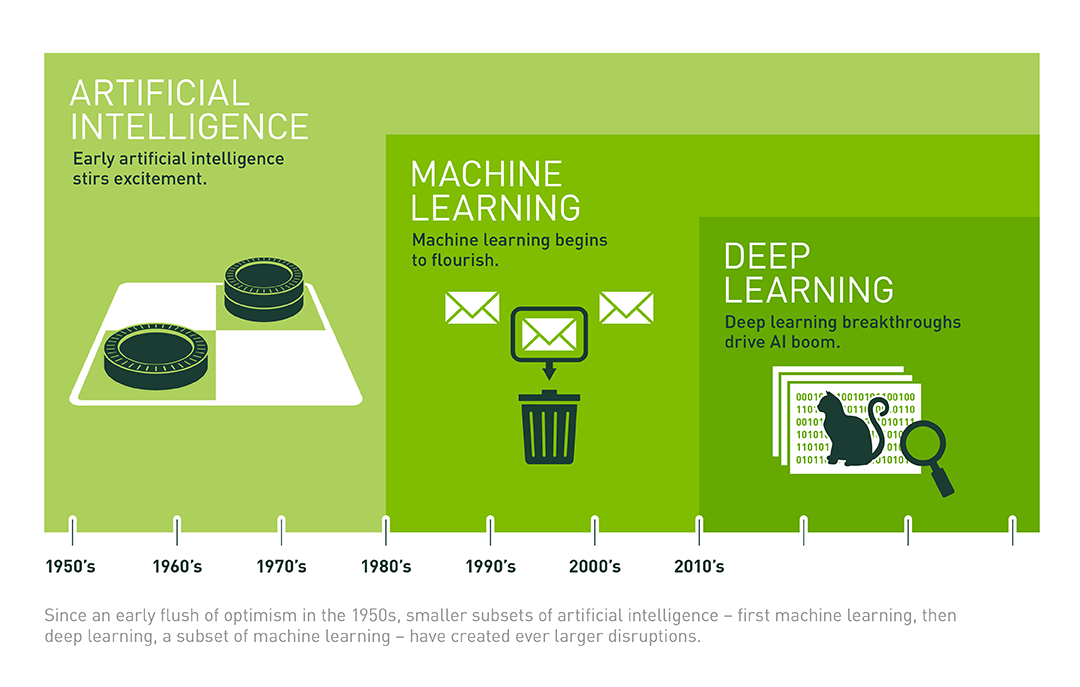
\includegraphics{evolution.png}}
	
	\end{frame}
	
	\begin{frame}[fragile]
	\frametitle{Évolution de L'intelligence  Artificielle : Machine Learning}
	\begin{itemize}
		\item Le machine learning permet à une machine d’adapter ses comportements en se fondant sur 				l’analyse des données à sa disposition. Un robot peut ainsi apprendre à marcher en commençant par 			des mouvements aléatoires, puis en sélectionnant les mouvements lui permettant d’avancer.
	\end{itemize}
	\end{frame}
	
	\begin{frame}[fragile]
	\frametitle{Évolution de L'intelligence  Artificielle : Deep Learning}
	\begin{itemize}
		\itemsep1em
		\item Le deep learning est la branche du machine learning qui utilise comme modèles mathématiques 			les réseaux de neurones formels, eux-mêmes construits sur la représentation mathématique et 					informatique d’un neurone biologique, née en 1943.
		\item  Le Deep Learning est utilisé dans la voiture autonome  de Google : le réseau de  neurones 					classifie tout l’environnement pour éviter les obstacles ou s’arrêter au bon moment 
	\end{itemize}
	\end{frame}
	
	\begin{frame}[fragile]
	\frametitle{Évolution de L'intelligence  Artificielle}
	
	\centerline{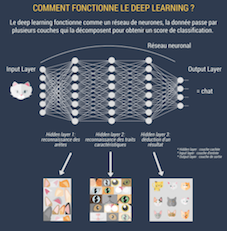
\includegraphics{deeplearning.png}}%changer pour image de meilleure qualitée
	
	\end{frame}
	
		\begin{frame}[fragile]
	\frametitle{Évolution de L'intelligence  Artificielle (fin)}
	\begin{itemize}
		\item Ces deux branches de l'intelligence artificielle ont causées de grandes améliorations de 						algorithmes, mais malgres cela l'IA d'aujourd'hui est est toujours qualifiée de « faible », en opposition 			à l’IA « forte » et consciente d’elle-même que prédisent les transhumanistes.

	\end{itemize}
	\end{frame}

\end{document}